\chapter{Traffic engineering in content-dominated ISP networks: background and motivation}
\label{ch:te-background}

This chapter serves two main purposes. First is to provide the reader with necessary background on ISP traffic engineering, content delivery and the interaction between traffic engineering and application-layer traffic adaptation (Section \ref{sec:bg-bg}). Second is to explain the motivation for our work on traffic engineering in content-dominated ISP networks in light of the existing work in this area (Section \ref{sec:bg-motivation}).




%In comparison, following are the main new research directions that we pursue in this thesis. We explain each of them further in the chapter.
%
%\begin{itemize}
%	\item
%	How do ISP traffic engineering schemes compare in terms of application-performance metrics such as TCP download time? Further, how do they compare while accounting fo r the effect of  application adaptation? 
%	\item
%	How should network CDNs--an ISP that operates a CDN on its infrastructure to deliver content to users on its network--perform content delivery given that they control both the content delivery and the underlying network routing?
%	\item
%	What role does content placement influence the interaction between network and content delivery, and what its its effect on user-perceived performance and netowrk cost?
%\end{itemize}


%Traffic engineering done by Internet service providers focuses on  computing the routing in the network for optimizing cost and other objectives. But, traffic engineering techniques are not isolated from mechanisms that alter the flow of traffic from the application. In particular, decisions at the application-layer ``overlay networks'' such as content placement and redirection also seek to alter how traffic flows in the network. Motivated by this observation, a question of long standing interest has been the following: 

%\emph{what influence do the decisions at the overlay have on the routing strategies of the underlying network, and vice versa?} 



%Internet is composed of independently controlled sub-networks called autonomous systems. an isp is one such autonomous system. an isp does traffic engineering to configure routing. in a content-dominated network, application-level decisions on content placement and request redirection affect traffic engineering. the high goal of this part of this thesis is to design and to evaluate traffic engineering schemes while accounting for the interaction with content delivery decisions. the focus on evaluating the role of content placement  while studying this interaction distinguishes us from prior work in this area.

%This chapter provides background on content delivery and traffic engineering and makes a case for studying the role of content placement on this interaction. Chapter x and Chapter y studies traffic engineering in two scenarios with varying degrees of flexiblity in placing content. Chapter x focuses on an ISP network in a fixed content placement scheme, namely that of placing content at multiple locations chosen randomly. While, Chapter y focuses on a network CDN, an ISP that deploys a CDN to deliver content to users on its network and enjoys full freedom to control the placement and routing on its network. 

\section{Background}
\label{sec:bg-bg}
Our review of prior work provides following main findings:

\begin{itemize}
	\item 
	ISP traffic engineering schemes compute routing for optimizing link-utilization based cost functions. These schemes commonly take a demand-aware approach that uses previously measured traffic matrics for computing future network routes (Section \ref{sec:ch2-te}).	
	\item 
	CDNs commonly use \emph{demand-oblivious} content placement and request redirection techniques towards improving user-perceived performance across the Internet (Section \ref{sec:ch2-cdn}). These techiques requires do not require content-level measurement of demand but instead use simple online heuristics to make their decision.
	\item 
	Prior work on the interaction between traffic engineering and application-layer adaptation focuses primarily on two aspects of application-layer adaptation --  overlay routing and request redirection. These interactions result in globally sub-optimal network cost as well as user-perceived latency, and co-operative mechanisms can leverage these interactions to improve cost and performance metrics.
\end{itemize}


\subsection{Traffic engineering}
\label{sec:ch2-te}

A key goal of ISP traffic engineering is to avoid congestion hotspots in the network by optimizing routes based on network topology and expected traffic demand that is represented in the form of traffic matrix. In ISP networks, traffic engineering decides both intra-domain routing (within the ISP) and inter-domain routing (across ISPs). We focus here on intra-domain routing and refer the reader to  \cite{Feamster2003,rexford} for a survey of inter-domain traffic engineering. 

The evaluation metric for ISP traffic engineering is a cost function that is dependent on the utilization of network links. A well-known cost function is maximum link utilization or MLU. A low link utilization is desirable to ISPs for two reasons. First, a low utilization of all links implies that the network is free from congestion hotspots. Second, it also implies that a network has more spare capacity to tolerate an increase in demand. Consider MLU as a capacity metric for example. If a traffic engineering scheme achieves an MLU of 0.25 for a given matrix, then it can tolerate up to a 4$\times$ surge in the load represented by the matrix.

We give an example to show how traffic engineering reduces link utilization. In Figure \ref{fig:te-example}, there are two links of capacity 1 Mbps and 3 Mbps between nodes A and B. The traffic from A to B is 2 Mbps. If a shortest path routing is followed, all traffic must be sent through either of the two links. The least MLU = 0.67 is achieved by using the large capacity link. A more flexible routing approach is to split traffic among the two links. Such a flow-split routing achieves MLU = 0.5 by sending 0.5 Mbps and 1.5 Mbps via the two links respectively. Thus, a better engineered routing resulted in a lower MLU in this example.

\begin{figure}
	\centering
	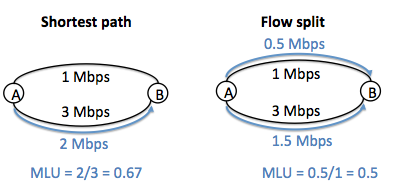
\includegraphics[scale=0.6]{fig/te-example.png}
	\caption{A flow-split routing reduces the maximum link utilization (MLU) over shortest-path routing.}
	\label{fig:te-example}
\end{figure}


If the traffic matrix is known accurately, the optimal solution to the traffic engineering problem can formulated as a multi-commodity flow optimization. The routing thus computed is refered to as \emph{optimal traffic engineering} in literature. As it is impossible to have accurate knowledge of future traffic matrices, traffic engineering schemes either take a \emph{demand-aware} or a \emph{demand-oblivious} approach. A demand-aware  traffic engineering  periodically updates routing using historically observed traffic matrices. A demand-oblivious  traffic engineering  requires no explicit measurement of traffic matices, but instead configures routing statically. A demand-oblivious  traffic engineering  is simpler to implement because it requires neither measuremnt nor periodic updating of network routing. 

%As it is impossible to have accurately knowledge of future traffic matrices. Therefore, practical traffic engineering schemes either take a demand-aware or a demand-oblivious approach.  A demand-aware  traffic engineering  periodically updates routing using historically observed traffic matrices. A demand-oblivious  traffic engineering  requires no explicit measurement of traffic matices, but instead configures routing statically. A demand-oblivious  traffic engineering  is simpler to implement because it requires neither measuremnt nor periodic updating of network routing. But, demand-aware schemes have been shown to outperform demand-oblivious  traffic engineering.

In practice, demand-aware traffic engineering based on Open Shortest Path First (OSPF) and Multiprotocol Label Switching (MPLS) are commonly used  \cite{COPE,MultiTM,fortz2000internet,MPLS2}. Routes computed by OSPF traffic engineering must follow shortest-weight paths, therefore OSPF TE provides limited functionality to split traffic among multiple paths. MPLS TE overcomes this limitation by enabling traffic between two nodes to be split  in arbitrary ratios among multiple paths. Therefore, MPLS TE gives better results than OSPF TE as exemplified above \cite{COPE,MultiTM}.

%Therefore, TE schemes commonly take a demand-aware approach, i.e., they compute routing using historically observed traffic matrices. In contrast, demand-oblivious simpler schemes also exist, no measurement of traffic matrix or continual updating of configuration. 

%But, future demand is not known perfectly. So, TE schemes commonly take a demand-aware approach: use historic demand patterns to predict future demand. In contrast, demand-oblivious simpler schemes also exist, no measurement of traffic matrix or continual updating of configuration. Demand-oblivious is simpler but demand-aware schemes have been shown to outperform them in TE literatue.

%
%Cost-based metrics: ignored the impact on end-user performance. So, what is the impact on end-user performance.
%
%TE is isolation, ignoring the internation with content placement and redirection.
%
%How do TE schemes compare when accounting for the interaction with content delivery.


\subsection{Content delivery}
\label{sec:ch2-cdn}

Content delivery systems seek to improve user-perceived performance for content accesses in all regions  at all times. A canonical example of a content delivery system is a content delivery network (CDN). State-of-the-art CDNs operate geo-distributed datacenters, and use a combination of edge caching, intelligent request redirection, and path and protocol optimizations for delivery of several types of content, e.g., video, bulk downloads, and interactive websites \cite{DilleyMPPSW02,akamai-overview}. Given their geo-distributed deployment, the decisions of content placement, i.e., locations at which acontent is placed, and request redirection, i.e., which location is best positioned to serve a user's request, are central to the functioning of a CDN.

\textbf{Content placement:} Content placement in CDNs is commonly done using caching schemes. For example a commonly used caching scheme is least recently used (LRU) cache replacement. There are two reason why content cahing is widely used. First, caching naturally captures geographic and temporal locality in content requests to populate caches with content likely to be reused. Second, a vast majority of network traffic is generated by content that gets updated infrequently, e.g., a video, audio, images. As a result, cached copies of content remain reusable for long duration. 

%Strong consistency is a separate topic and is studied in the content of design of geo-distrbuted kv store in auspice.\tbd{fix this}

\textbf{Request redirection:} In a CDN, request rediection occurs at two tiers - inter-datacenter and intra-datacenter. Our focus in this part of the thesis is on inter-datacenter request redirection because it influences wide-area traffic patterns that affect traffic engineering. We discuss intra datacenter redirection in the context of a Content Datcenter (Chapter \ref{ch:shrink}).

Request redirection strategies complement placement strategies by selecting the server location that is best suited to process a user's request. These strategies have been extensively studied and form the heart of CDN technology today. To quote from a report by Akamai,  \emph{``the system directs client requests to the nearest available server likely to have the requested content."} where the ``nearest" server is one whose round trip latency as well as packet losses are small, and  an ``available" server is one that has sufficient resources to serve a request \cite{DilleyMPPSW02}. 

Request redirection is implemented using three processes: (1) \emph{Monitoring:} Probe messages sent intermittently help monitor network characteristics and server load and identify congested regions of network and overloaded server locations \cite{oasis,donar}. (2) \emph{Estimating distances:} The measured statistics are combined to compute a distance function that reflects the proximity of a server location to users in a geographic region \cite{donar}. (3) \emph{Informing the user:} The user is informed of selected server/s either via DNS resolution \cite{DilleyMPPSW02} or via HTTP redirection \cite{barbir2003known}.

Content delivery techniques can be classified into demand-aware and demand-oblivious similar to our classfication of traffic engineering schemes. We consider common content delivery techniques discussed above to be demand-oblivious since they do not require long term content-level measurement of demand but instead use simple online heuristics to make their decision.. In contrast, a demand-aware approach to  placement and redirection has also been studied, e.g., Applegate \emph{et al.} use a demand-aware approach to determine placement and redirection for Video-on-Demand content in the network. 

\subsection{Interaction between traffic engineering and application-layer adaptation}
\label{sec:ch2-te-cdn}

Studying the interaction between network-layer routing computed by traffic engineering and application-layer adaptation has been a topic of long standing interest in computer science. Several related questions have been put forth. Does this interaction yield globally sub-optimal results? How can we design cooperative mechanisms to leverage these interactions? Do cooperative mechanisms yield benefit in an Internet-like environment? Most previous research on this topic has focused on the interaction of traffic engineering with either overlay routing \cite{Roughgarden,selfishQiu} or with request redirection \cite{Jiang2009,JohariGameTheory, CATE, P4P} as discussed below. 

\textbf{Interaction between traffic engineering and overlay routing:} Several results show the negative interaction between selfish overlay routing and network routing \cite{Roughgarden,selfishQiu}. Theoretical results indicate that the negative interaction could cause an arbitrary degradation in user perceived delay. Further studies using Internet-like traffic demands and topologies indicate that this interaction hurts traffic engineering metrics. While this body of work focuses on application adaptation to \emph{path diversity} created by overlay routing, our work focuses on \emph{location diversity} present in the Internet (Chapter \ref{ch:beyondmlu}). We do not consider overlay routing since our focus is primarily on intra-domain routing while overlay routing is most commonly used to mask inter-domain routing inefficiencies. 


\textbf{Interaction between traffic engineering and request redirection:} Recent work has studied the interaction between ISP traffic engineering and request redirection by content providers with geo-distribtued datacenters as well as P2P applications. Both analytical results \cite{Jiang2009,JohariGameTheory} and system implementations \cite{CATE,P4P} have shown that there is value for joint optimization of request redirection and traffic engineering, and cooperative strategies can help traffic engineering metrics while maintaining or improving user-perceived performance. Our work distinguishes in that  we model the three-way interaction between placement, redirection and routing and show that placement flexibility is more powerful degree of freedom than redirection or routing to improve traffic engineering metrics and to reduce user-perceived latency (Chapter \ref{ch:ncdn}).


\section{Motivation}
\label{sec:bg-motivation}

A content-dominated traffic and the presence of content at multiple network locations changes the traditional ISP traffic enginering problem. In such a network, a traffic matrix is no longer an effective representation of demand. It can be changed via application-layer adaptation without any underlying change in demand as we demonstrate in this section. Demand is better expressed as a \emph{content matrix} in which each entry represents the demand for a content at a particular network location. A traffic matrix implicitly assumes a fixed source and a fixed destination for each traffic flow. But, a content matrix expresses the fact that the demand for a content at a particular destination can be served from any set of source locations. As we explain using examples below, the flexibility of serving the demand from any location raises questions on the usefulness of link-utilization based metrics that are commonly used in traffic engineering (Section \ref{sec:bg-poormlu}) as well on the importance of traffic engineering itself (Example \ref{sec:bg-ncdn-interaction}). These and other related questions motivate our work on traffic-engineering in content dominated networks.

Our work presents research on two network scenarios that vary in terms of application adaptation mechanism and the content placement flexibility in the network. We explain the two scenarios and motivate the research questions we address in each case using examples.

\subsection{ISP network with content location diversity}
\label{sec:bg-locdiv}
We consider an ISP network that has little control over placement and redirection, but applications can leverage \emph{location diversity}, or  the ability to download content from multiple locatioons. We motivate why traffic engineering schemes must be evaluated while accounting for their interaction with location diversity, and why we need to look beyond link-utilization based metrics in evaluating traffic engineering schemes. These questions are addressed in Chapter \ref{ch:beyondmlu}.

\subsubsection{Interaction between traffic engineering and location diversity}
\label{sec:bg-3node}

\begin{figure}[tbh]
	\centering
	\label{fig:3node-bg}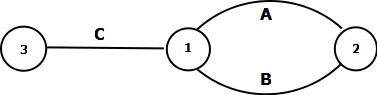
\includegraphics[scale=0.5]{final_images/Diagram3node.png}
	\caption{Lasso network}
\end{figure}

This example illustrates how location diversity can change the traffic matrix without any underlying change in demand. In Figure~\ref{fig:3node-bg}, all links are assumed to have a capacity of 100 units and a constant delay. The top link A has a very small delay compared to the other two links that both have equal delay. Node 1 has 100 Mbps of demand that it can obtain from 2 as well as 3. In addition, there is 20 Mbps of demand at node 1 which it can obtain only from 2.  We assume that the aggregate demand at a node consists of a large number of user-initiated connections. When content can be downloaded from multiple locations, users initiate parallel TCP connections and the throughputs along paths in a parallel TCP connection are inversely proportional to the path delays. The TE scheme is assumed to be OSPF-based, i.e., shortest-path routing using configured link weights and traffic split equally among multiple paths with equal weights.

Suppose the weights of the links A and B are unequal and the link A has more weight. As a result, all of the traffic between 1 and 2 is routed using only link B. 1 splits its demand of 100 Mbps using parallel TCP equally between links B and C. Thus, the traffic on links A, B, and C is  0, 70, and 50 respectively. In the next step, seeking to balance load better for this resultant matrix, the TE scheme sets both the links A and B to the same weight (hoping to achieve link utilizations of 35, 35, and 50 respectively).  Consider how parallel TCP connections respond to this change. Assuming each TCP connection between 1--2 is pinned to only one of the two paths---as is commonly done in practice to achieve equal-cost multi-path (ECMP) splitting---50 Mbps of demand at 1 gets routed using parallel TCP connections over the link A and link C, and an equal amount using parallel TCP connections along the link B and link C. In addition, the 20 Mbps of background traffic is split equally among link A and link B as per ECMP.  Since link A has a much smaller delay than link C, the 50 Mbps of demand at 1 using parallel TCP along those two paths will flow entirely through link A. The remaining 50 Mbps using B and link C will get split equally across the two paths by parallel TCP. Thus, the traffic on the links A, B and C is 60, 35, and 25 respectively, which is different from what the TE scheme engineered for (namely, 35, 35, and 50). The resulting MLU of 0.6 is different compared to 0.5, the value that the TE scheme expected. This example illustrates that the outcome of traffic engineering depends on the application adaptation to location diversity, thereby motivating us to study the following question.

\emph{Research question: How do traffic engineering schemes compare while accounting for the effect of location diversity in the network?}

\subsubsection{Shortcomings of link-utilization metrics}
\label{sec:bg-poormlu}

%We explain why link-utilization based metrics may not reflect user-perceived performance. Further, they are a poor metric to measure network capacity, i.e., the factor of surges in traffic demand that a network can tolerate, in a network with location diversity.

Link-utilization based metrics may not be a good predictor of user-perceived performance that depends on other factors such as propagtion delay, access link capacity and backbone link capacity also. Moreover, queuing-theoretic models show that only a high link utilization severely affects performance-critical metrics such as queuing delay and packet loss. For low to moderate link utilization that is common in today's ISPs, a reduction in link utilization may not yield a commensurate benefit in application peformance. 

\emph{Research question: Are link-utilization based metrics good predictors of user-perceived performance for real network topologies and traffic matrices?}

Link-utilization based metrics such as MLU are poor metric for network capacity in the presence of location diversity. Unfortunately, as the example in Figure \ref{fig:3node-bg} shows, MLU is not a meaningful metric of capacity when application adaptation to location diversity determines the traffic matrix. 
Thus, location diversity necessitates a new capacity metric.

%Link-utilization based metrics may not be a good predictor of network capacity in scenarios where applications have the ability to download content from mulitple locations. We illustrate this point using an example. \tbd{complete the example, add figure}

\emph{Research question: How do we quantify network capacity under location diversity?}

\subsection{Network CDN}
\label{sec:bg-ncdn}
Network CDNs are a recent, potentialy transformative trend in which ISPs deploy CDNs on their infrastructures to deliver content to users on their network.  Unlike traditional ISPs and traditional CDNs, NCDNs enjoy full control over placement, redirection and routing on their networks. The interaction between placement and routing in an NCDN illustrated below motivates us to explore the benefit of joint optimization of placement, redirection and routing as well as to evaluate the relative importance of placement and routing in an NCDN. These questions are addressed in Chapter \ref{ch:ncdn}.

\subsubsection{Interaction between placement and routing in an NCDN}
\label{sec:bg-ncdn-interaction}

To appreciate how placement can shape traffic in an NCDN, consider the simple example in Figure~\ref{fig:NetworkExample}. Node $C$ has an object in its cache that is requested by end-users at nodes $A$ and $D$. Suppose that one unit of traffic needs to be routed from $C$ to $A$ and $0.5$ units  from $C$ to $D$ to satisfy the demand for that object. The routing that achieves the minimum MLU of $0.5$ to serve the demanded object is shown in the figure. Note that the routing that achieves the MLU of 0.5 is not possible with a simple, \unplanned\ scheme like hop-count as that would route all the traffic demand from $C$ to $A$ via $B$, resulting in an MLU of 1. Thus, a (\planned) traffic engineering scheme is necessary to achieve an MLU of 0.5.

\begin{figure}[h]
	\centering
	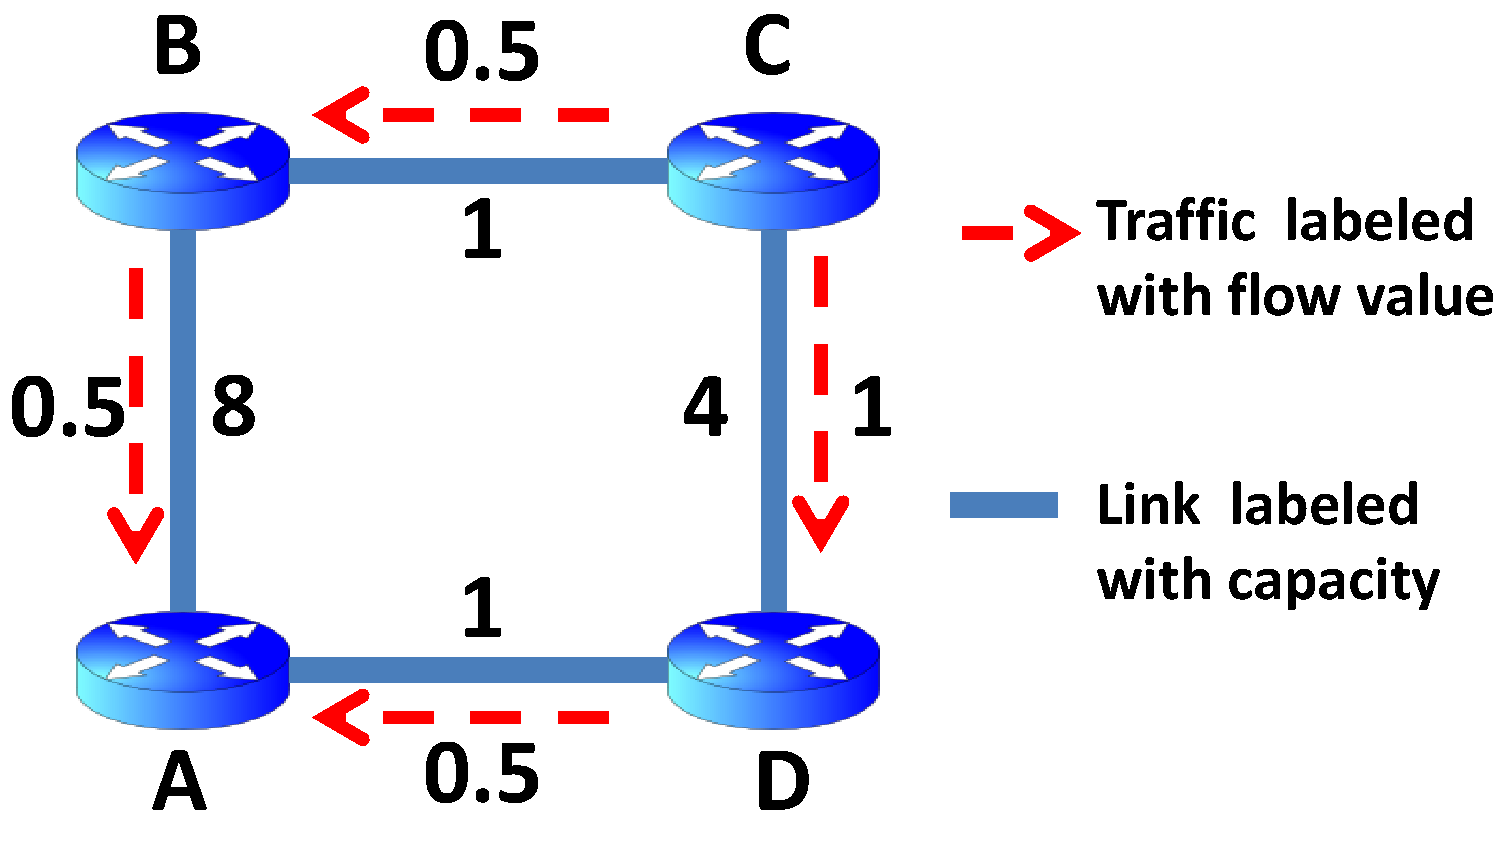
\includegraphics[width=2in]{ncdnpaper/ncdn-example}
	\caption{A simple \ncp\ example}
	\vspace{-.3in}
	\label{fig:NetworkExample}
\end{figure}

On the other hand, NCDNs can shape the traffic demand matrix by using a judicious placement and redirection scheme. Suppose that there is some space left in the content server's cache at node $B$ to accommodate an additional copy of the demanded object. By creating an additional copy of the object at $B$, the traffic demand of $A$ can be satisfied from $B$ and the demand of $D$ from $C$ achieving an MLU of $0.125$. In this case, judicious content placement decreased the MLU by a factor of $4$. Even more interestingly, this best MLU can be achieved using a simple routing scheme like hop-count routing while also improving user-perceived latency (assuming that the latency of link $BA$ is lower than that of the two-hop paths from $C$ to $A$). While this is a toy example, it shows that content placement flexibility reduces network cost and enables simpler routing. This interaction between placement and routing motivates us address the following questions for real content workloads and network topologies. 

\emph{Research question: Does a joint optimization of placement, redirection and routing yield benefits over independently making these decisions using simple demand-oblivious schemes?}

\emph{Research question: Does content placement flexibility obviate sophisticated traffic engineering in an NCDN?}




%A Network CDN (NCDN) is an ISP than owns and operates a CDN over its infrastructures to deliver content to its end users. As NCDNs manage both the underlying network and content delivey, the objectives and the techniques available to a network CDNs are not the same from a traditional ISP or a tradidional CDN. Our work is motivated by the following questions:
%
%\begin{itemize}
%	\item 
%	Is a demand-aware or a demand-oblivious content delivery and traffic engineering scheme more effective for a network CDN?
%	\item
%	An NCDN can potentially jointly optimize content delivery and traffic engineeing, but do such sophisticated schemes yield benefits from a CDN?
%\end{itemize}
%
%To our knowledge, this thesis presents the first study of techniques for a managing a NCDN based on real network topology and content access traces. Our result show the effectiveness of simple demand-oblivious schemes for content delivery and traffic engineering in achieving performance close to an ideal scheme. Further, they show that a demand-aware joint optimization performs poorly due to frequnt churn in content workloads and change in access patterns. 





